Considereu la funció definida a trossos següent:
\[
f(x)=\begin{cases}
  5e^{2x} & \si{x\le 0},\\[3pt]
  (x+m)^2+1 & \si{0<x<2},\\[3pt]
  1 & \si{2\le x},
\end{cases}
\]
on $m$ és un paràmetre real.

\begin{apartats}

\apartat{1}
Determineu els valors de $m$ que fan que la funció $f(x)$ sigui contínua en tot el seu
domini. Justifiqueu la resposta.

\begin{solucio}
Com que les tres funcions que defineixen $f$ són contínues en els seus respectius
intervals de definició, només cal imposar que $f$ sigui contínua als punts de contacte,
$x=0$ i $x=2$.\\
En $x=0$: $\lim_{x\to0^-}f(x)=\lim_{x\to0^-}5e^{2x}=5$, \ $f(0)=5e^0=5$ \ i
$\lim_{x\to0^+}f(x)=\lim_{x\to0^+}\big((x+m)^2+1\big)=m^2+1$. Per tant, $f$ és contínua en
$x=0$ si i només si $m^2+1=5$, cosa que passa si i només si $m=\pm2$.\\
En $x=2$: $\lim_{x\to2^-}f(x)=(2+m)^2+1$, \ $f(2)=1$ \ i $\lim_{x\to2^+}f(x)=1$, i la funció
és contínua en $x=2$ si i només si $(2+m)^2+1=1$, cosa que passa si i només si $m=-2$.\\
Per tant, la funció és contínua en tots els punts \textbf{només quan $m=-2$}.

\textit{Pauta oficial:} 0,25 per justificar que ja és contínua fora dels punts de
contacte; 0,25 per estudiar cadascun dels dos contactes, i 0,25 per combinar-ho i donar
la resposta final correcta.
\end{solucio}

\apartat{1}
Feu un esbós de la gràfica de $y=f(x)$ per al cas $m=-2$, i calculeu l'àrea delimitada
per aquesta gràfica, l'eix $OX$ i les rectes $x=-1$ i $x=3$.

\begin{solucio}
\begin{center}
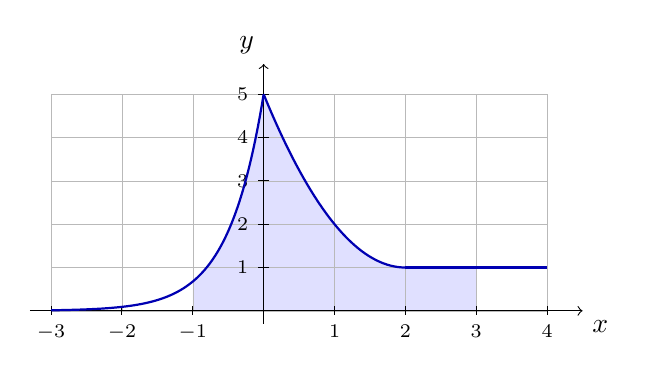
\begin{tikzpicture}[x=0.9cm,y=0.55cm]
  \fill[blue!12,domain=-1:0,samples=40] (-1,0) -- plot (\x,{5*exp(2*\x)}) -- (0,0) -- cycle;
  \fill[blue!12,domain=0:2,samples=40] (0,0) -- plot (\x,{(\x-2)^2+1}) -- (2,0) -- cycle;
  \fill[blue!12] (2,0) rectangle (3,1);
  \draw[gray!55,very thin,step=1] (-3,0) grid (4,5);
  \draw[->] (-3.3,0) -- (4.5,0) node[below right] {$x$};
  \draw[->] (0,-0.3) -- (0,5.7) node[above left] {$y$};
  \foreach \i in {-3,-2,-1,1,2,3,4} \draw (\i,0.1) -- (\i,-0.1) node[below,font=\scriptsize] {$\i$};
  \foreach \j in {1,2,3,4,5} \draw (0.08,\j) -- (-0.08,\j) node[left,font=\scriptsize] {$\j$};
  \draw[blue!70!black,thick,domain=-3:0,samples=80,smooth] plot (\x,{5*exp(2*\x)});
  \draw[blue!70!black,thick,domain=0:2,samples=40,smooth] plot (\x,{(\x-2)^2+1});
  \draw[blue!70!black,thick] (2,1) -- (4,1);
\end{tikzpicture}
\end{center}
Per representar la funció quadràtica es pot calcular el vèrtex amb la fórmula
$x=\frac{-b}{2a}=2$, o bé observar que és una translació 2 unitats a la dreta i una unitat
amunt de la paràbola $y=x^2$.\\
És clar, fins i tot sense la gràfica, que la funció és positiva en tot el seu domini. Per
tant, per calcular l'àrea demanada cal calcular la integral definida
\begin{align*}
A&=\int_{-1}^{3}f(x)\,dx=\int_{-1}^{0}5e^{2x}\,dx+\int_{0}^{2}\big((x-2)^2+1\big)\,dx+\int_{2}^{3}1\,dx\\
 &=\Big[\tfrac52\,e^{2x}\Big]_{-1}^{0}+\Big[\tfrac{(x-2)^3}{3}+x\Big]_{0}^{2}+\Big[x\Big]_{2}^{3}
  =\frac52-\frac{5}{2e^2}+2+\frac83+3-2\simeq7{,}83\ \text{u}^2.
\end{align*}
\textit{Pauta oficial:} 0,25 per l'esbós de la gràfica; 0,25 pel plantejament correcte de
l'àrea com a suma d'integrals; 0,25 pel càlcul de la integral de la part exponencial, i
0,25 per la integral de la part parabòlica.
\end{solucio}

\apartat{0,5}
Per a $m=-2$, trobeu un punt on la recta tangent a $y=f(x)$ sigui paral·lela a $y=-2x$.
Calculeu l'equació d'aquesta recta tangent.

\begin{solucio}
Com que el primer tram de la gràfica és creixent, i el tercer és pla, només pot haver-hi
punts amb pendent negativa al tram del mig. Volem un punt on el pendent sigui $-2$; per
tant, derivem el tram parabòlic i igualem la derivada a $-2$:
$2(x-2)=-2\ \Rightarrow\ x=1$.\\
La recta tangent al punt $\big(1,f(1)\big)=(1,2)$ és $y-2=-2(x-1)$, és a dir, $y=-2x+4$.

\textit{Pauta oficial:} 0,25 per trobar el punt i 0,25 pel càlcul de l'equació de la recta
tangent.
\end{solucio}

\end{apartats}
